% =====================================================================
\chapter{Notação Θ: o crescimento exato}\label{cap:07}
\naaula{25 a 27}

Quando uma função tem o mesmo $g$ como teto \emph{e} como piso, sabemos exatamente como ela
cresce. É isso que a notação $\Theta$ (lê-se \enquote{teta grande}) expressa.

\section{A definição}

\begin{center}
\colorbox{edtealclaro}{\parbox{0.92\textwidth}{\centering\large
$f(n) = \Theta(g(n))$ \ se existem constantes $c_1 > 0$, $c_2 > 0$ e $n_0 \ge 1$ tais que\\[0.3em]
$c_1 \cdot g(n) \;\le\; f(n) \;\le\; c_2 \cdot g(n)$ \ para todo $n \ge n_0$.}}
\end{center}

Em outras palavras: $f(n) = \Theta(g(n))$ quando $f(n) = O(g(n))$ \textbf{e} $f(n) = \Omega(g(n))$.
A função fica \enquote{ensanduichada} entre dois múltiplos de $g$.

\begin{figure}[!htb]
  \centering
  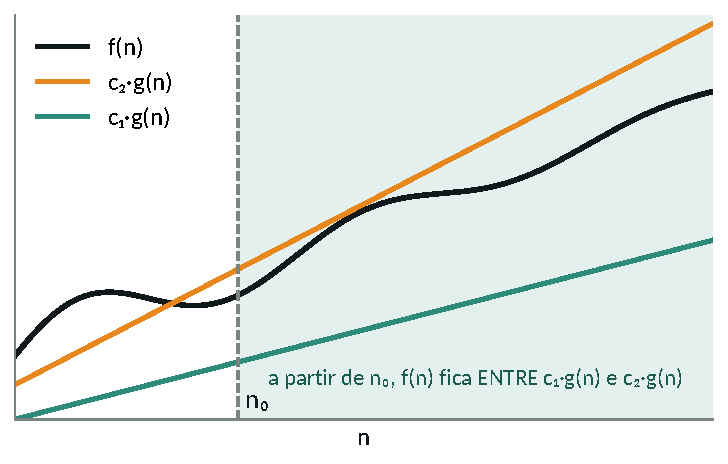
\includegraphics[width=0.72\textwidth]{figuras/f07_definicao_Theta.pdf}
  \caption{A partir de $n_0$, $f$ fica presa na faixa entre $c_1 \cdot g(n)$ e $c_2 \cdot g(n)$.}
\end{figure}

\section{Exemplos}

\textbf{$3n + 4 = \Theta(n)$.} Já temos as duas metades: no capítulo 5, $3n + 4 \le 4n$ para
$n \ge 4$; no capítulo 6, $3n + 4 \ge 3n$ para $n \ge 1$. Juntando, com $c_1 = 3$, $c_2 = 4$ e
$n_0 = 4$ (o maior dos dois $n_0$):
\[
3n \;\le\; 3n + 4 \;\le\; 4n \qquad \text{para todo } n \ge 4.
\]

\textbf{$n^2 + n = \Theta(n^2)$.} Para $n \ge 1$: $n^2 \le n^2 + n$ (óbvio) e
$n^2 + n \le n^2 + n^2 = 2n^2$. Então $c_1 = 1$, $c_2 = 2$ e $n_0 = 1$.

\section{Resumo das três notações}

\begin{center}
\begin{tabularx}{\textwidth}{P{1.6cm} P{2.6cm} P{2.6cm} P{3.3cm} L}
\cab \tc{Notação} & \tc{Lê-se} & \tc{Ideia} & \tc{Desigualdade} & \tc{Como comparar números} \\
$O(g)$ & ó grande & teto & $f \le c \cdot g$ & como \enquote{$\le$} \\
\rowcolor{edfundo} $\Omega(g)$ & ômega grande & piso & $f \ge c \cdot g$ & como \enquote{$\ge$} \\
$\Theta(g)$ & teta grande & crescimento exato & $c_1 g \le f \le c_2 g$ & como \enquote{$=$} \\
\end{tabularx}
\end{center}

\begin{intuicao}
A comparação com números ajuda a lembrar: dizer $f = O(g)$ é como dizer \enquote{a velocidade de
crescimento de $f$ é $\le$ a de $g$}; $\Omega$ é \enquote{$\ge$}; e $\Theta$ é \enquote{$=$}.
Sempre em termos de \emph{forma de crescimento}, ignorando constantes.
\end{intuicao}

\section{Uma regra prática para polinômios}

Se $f(n)$ é um polinômio cujo maior expoente é $d$ e o coeficiente desse termo é positivo, então
$f(n) = \Theta(n^d)$. Exemplos: $3n + 4 = \Theta(n)$; $3n^2 + 4n + 2 = \Theta(n^2)$;
$\dfrac{n(n-1)}{2} = \Theta(n^2)$. É a formalização exata da ideia de termo dominante do
capítulo 4.

\begin{conexao}
Agora dá para dizer com precisão alguns custos das aulas anteriores:
\begin{itemize}
  \item \codigo{empilhar()}, \codigo{desempilhar()} e \codigo{consultar_topo()} da Pilha: $\Theta(1)$.
  \item \codigo{enfileirar()} e \codigo{desenfileirar()} da Fila com ponteiro para o fim: $\Theta(1)$.
  \item \codigo{percorrer()} de qualquer Lista com $n$ elementos: $\Theta(n)$.
  \item Inserir $n$ elementos, um a um, no início de uma lista contígua: $\dfrac{n(n-1)}{2}$
        deslocamentos, ou seja, $\Theta(n^2)$.
\end{itemize}
\end{conexao}

\begin{exrapido}
(a) Mostre que $3n + 4 = \Theta(n)$, dando $c_1$, $c_2$ e $n_0$. (b) Mostre que
$4n^2 - 10n + 7 = \Theta(n^2)$. (Dica para o piso: $7 \ge 0$ e \enquote{gaste} metade do $4n^2$
com o $-10n$.)
\end{exrapido}

\begin{respostas}
  \resp{7.1} (a) $c_1 = 3$, $c_2 = 4$, $n_0 = 4$ (seção 7.2).
  (b) \emph{Teto:} para $n \ge 1$, $-10n \le 0$ e $7 \le 7n^2$, então $4n^2 - 10n + 7 \le 4n^2 + 7n^2 = 11n^2$.
  \emph{Piso:} como $7 \ge 0$, temos $4n^2 - 10n + 7 \ge 4n^2 - 10n$, e
  $4n^2 - 10n \ge 2n^2 \Longleftrightarrow 2n^2 \ge 10n \Longleftrightarrow n \ge 5$.
  Logo, $c_1 = 2$, $c_2 = 11$ e $n_0 = 5$.
\end{respostas}
